\documentclass[a4paper,twoside]{article}
\usepackage[utf8]{inputenc}
%\usepackage[uebung, answers]{tumbgdm}
\usepackage[klausur]{tumbgdm}
\Professor{Prof. Dr. Martin Werner}
\Universitaet{Technical University of Munich}
\Institut{School of Engineering and Design}
\Lehrstuhl{Professorship Big Geospatial Data Management}
\Semester[WiTe 2021/22]{Winter Term 2021/22}
\Vorlesung{Computational Foundations I}
\InstitutsWebsite{https://www.bgd.lrg.tum.de/}
\VorlesungsWebsite{https://www.moodle.tum.de/course/view.php?id=72588}
\usepackage{pdfpages}
%\nummerUebungsblatt{6}
%\nummerErsteFrage{14}
\klausurTitle{2nd Exam Computational Foundations I \\(LRG0060, WS 2021/22)}
%\LearningOutcome{
%We are warming up with C/C++ programming environments.
%}
\lstset{numbers=left, stepnumber=1}
\begin{document}

\maketitle
% 90 points for 90 minutes
\evaluationtable

\clearpage

\begin{task}{Multiple Choice}{5}{}
  Answer the following questions with yes or no. \\
  \emph{A wrong answer is counted as -1, a correct answer is counted as +1, an answer not given is counted as 0 (if you don't know the answer it is smarter not to give an answer!). If you reach more than 5 points, the points will become bonus points, if you reach less than 0 points, the result is 0 points.}
  \vspace{2cm}
  
\begin{mclist}
  \mcquestion{In C++, objects can be allocated with \texttt{new}. In order to release them, one uses the function \texttt{free}.}{}{X}{}
 \mcquestion{A Markov algorithm can not be implemented on a Turing machine.}{}{X}{}
 \mcquestion{For arbitrary large $n$, an algorithm of runtime complexity $O(n^2 )$ will become faster than an algorithm of $O(n)$.}{}{X}{Of course}
 \mcquestion{The SDL libraries allow for visualizing things from C++.}{}{X}{SDL = Simple Direct Media Layer = simple GUI framework.}
 \mcquestion{MATLAB is an interpreted language. Hence, MATLAB code runs typically faster than code written in a compiled language.}{}{X}{}
 \mcquestion{C++ is an extension to C.}{X}{}{}
 \mcquestion{A binary tree with depth $n$ has at most $\sum_{l=0}^{n-1} 2^l$ nodes.}{X}{}{}
  \end{mclist}

   


\end{task}
\clearpage
\begin{task}{Algorithm Representation}{5}{}
  Consider the Algorithm in Listing \ref{lst:listing1}
  \begin{lstlisting}[caption=An imperative program, label=lst:listing1]
    DECLARE A,B,C,D,E,RESULT
    A = 4;
    B = SQUARE(A);
    C = 2;
    D = 5;
    E = C+D;
    RESULT = E*B;
\end{lstlisting}

  \begin{enumerate}
  \item {Write a table with a row for each line of the previous program and a column for each variable declared and give the value \textbf{after} the line has completed. Use a ? if the value is unknown (e.g., the variable has not yet been initialized). Include Line 1 (which just means every variable value is unknown).
    \vspace*{8cm}}
    \clearpage
    
  \item{Consider the following program:
\begin{lstlisting}
A = CIRCLE(P, R);
B = CIRCLE(Q, R);
M1, M2 = INTERSECT(A,B);
L = LINE(M1,M2)
RESULT = INTERSECT(L, LINE(P,Q))
\end{lstlisting}


    Give the same program as a single expression for result. That is, not using multiple lines of imperative code, but braces to organize the computation of the result.
    \vspace*{4cm}}

  \item{Assume P, Q are given points, R is the radius of the circles and the length of the segment from P to Q, INTERSECT returns two intersection points of geometries (either of two circles or of two lines), LINE constructs a line between two points. Draw what the program does. Give variable names as labels for the objects you draw.\vspace*{2cm}}

    
  \end{enumerate}
  
  
\end{task}
%\clearpage
%
%\begin{task}{Turtle Graphics}{5}{}
%  Consider a turtle with commands \code{m} for move, \code{l} for turn left by $90^\circ$ and \code{r} for turning right. The turtle starts in the marked position.
%  
%  \centering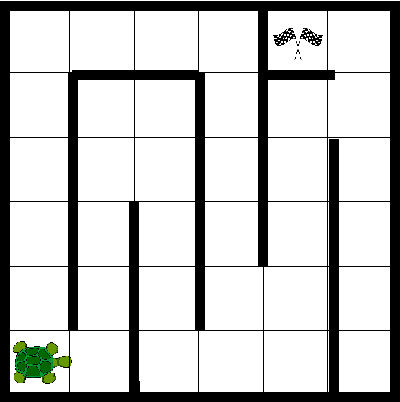
\includegraphics[width=.4\textwidth]{gfx/turtlemaze.pdf}
%
%  \begin{enumerate}
%  \item{Sketch an imperative program that gets the turtle into the goal location not crossing bold walls. Denote the program as a string consisting of aforementioned characeters. For example \code{ml} means move and then turn left.\vspace{2cm}}
%  \item{
%    Now, we add a simple sensor to our turtle: It is always able to check whether it can move forward by running a
%    C++ function \code{bool empty()}. In this context, the movement commands are implemented as C++ function \code{move()}, \code{turnleft()}, and \code{turnright()}. Give a short C++ program (without any function declaration, just the functional body) that solves the maze using \code{while} loops to avoid repetitions of commands. Write up to three columns - the program is not short.
%  }
%
%  \end{enumerate}
%
%
%\end{task}
%\clearpage
%MARK
\clearpage
\begin{task}{Program Analysis}{15}{}
  Consider the C++ program in Listing \ref{lst:clock}. The function print just outputs a space-separated list of the values of
  the argument vector and its implementation details can be ignored. 
  \lstinputlisting[caption=Nice Program, label=lst:clock]{code/clock.cpp}

  \begin{enumerate}
  \item{How often is the loop  executed?\vspace{2cm}}\clearpage
  \item{Give the complete output of the program.\vspace{12cm}}
  \item{Define the term ``Loop Variant'' in one sentence. Only the first given sentence is taken into account. \vspace{3cm}}
    \end{enumerate}
\end{task} % Give implementation, let students run it
\clearpage

\begin{task}{Turing Machine}{10}{}
  Given a Turing machine with a finite string of 0s and 1s on the tape, delimited in both directions with empties $\epsilon$,
  implement an algorithm that interprets the tape as an unsigned integer numbers and computes the increment.
  Implement the Turing machine with no more than three states, where the final state is called \code{done} and has no
  outgoing rules.

  \begin{enumerate}
  \item{Give the machine as a transition table. The table can be incomplete. As agreed, the machine will halt if there is no applicable rule. \vspace{10cm}}
  \item{Which of the following properties do Turing machines have? Answer yes or no:
    \begin{itemize}
    \item {they are determined: \vspace{1cm}}
    \item {they are deterministic:\vspace{1cm}}
    \item {they are capable of computing Markov Algorithms:\vspace{1cm}} 
    \end{itemize}
      }
  \end{enumerate}

  
  % for turingmachine.io
%input: '000100101011011100101010'
%blank: ' '
%start state: start
%table:
%  start:
%    1: {R: state_once}
%    0: {R: start}
%    ' '  : {R: notfound}
%  state_once:
%    1: {R: state_twice}
%    0: {R: start}
%    ' '  : {R: notfound}
%  state_twice:
%    1: {R: found}
%    0: {R: start}
%    ' '  : {R: notfound}
%  found:
%  notfound:
  \end{task}
  \clearpage
  
  \begin{task}{Markov Algorithms}{10}{}
    Markov algorithms have been introduced to simplify the analysis and implementation of Semi Thue Systems.
    

    \begin{lstlisting}[mathescape,caption=A Markov Algorithm]
|0 -> 0||
1 -> 0|
0 -> $\epsilon$
      \end{lstlisting}
    
    \begin{enumerate}
    \item {What is the key difference (1 sentence) between Semi Thue systems and Markov algorithms?\vspace{2cm}}
    \item{Execute the given Markov algorithm on the input strings ``101'' and ``11''. Give all intermediate strings and (preferably for correction) the line number of the rule you applied.
      Tip: Write your transitions below each other as most rules don't change the length. Mark the left hand side (e.g., underline), replace it, and fill in the rest. \vspace{6cm}}
      \clearpage
    \item{ In general,what does this program do? (One Sentence)
      }
    \end{enumerate}
\end{task}

  \clearpage
  \begin{task}{Understanding Recursion}{5}{}
    Consider the following program
    \lstinputlisting[caption="Recursion"]{code/recursion2.cpp}

    \begin{enumerate}
    \item{First, give all function calls with parameters (written like ``$A(4) \Rightarrow A(5) \Rightarrow B(2)$'') and the final value. Then, give the exact output of the program.\vspace{5cm}}
    \item{[2 Bonus Points] For which inputs does the function $A$ terminate? Give a short reason. Ignore possible overflow or underflows from finite arithmetic representation.\vspace{2cm}}

    \end{enumerate}
    

  \end{task}
  \clearpage
  \begin{task}{The Structured Program Theorem}{5}{}
    We introduced the Turing machine as a basic model for computing. However, programming of computers is
    not done in the language of Turing machines in practice. The Structured Program Theorem names three concepts that
    a programming language must fulfill to efficiently express all Turing programs.

    Name these three concepts and draw them as a flow chart.
    \end{task}
    \clearpage

%    \begin{task}{Object Orientation}{5}{}
%      Shorty answer the following questions on object orientation.
%      \begin{enumerate} 
%      \item{What is polymorphism\vspace{4cm}}
%      \item{What is the difference between a function and a \code{virtual} function?\vspace{2cm}}
%      \item{Why doesn't the following program compile?
%        \lstinputlisting[caption=Object Orietntation]{code/oo.cpp}\vspace{2cm}}
%      \item{What is the output if the error is corrected?\vspace{2cm}}
%        
%        
%        
%        \end{enumerate}
%
%
%    \end{task}
    \begin{task}{Composition and Recursive Data Structures}{5}{}
      In the lecture, we have learnt about recursive data structures.
      Declare a class in C++ which could be used to implement a binary tree. Give no methods except a constructor
      that ensures proper initialization of the needed pointer variable.
      (The answer will typically have less than 10 lines, we are not picky about syntax.
      If it is semantically sensible, you get all points!) \vspace{6cm}
    \end{task}
    \clearpage
    \begin{task}{Faculty}{10}{}
      Sketch two implementation (we don't care about syntactic details) of a function that calculates the sum
      \[
          \sum_{i=0}^{N} 2\cdot i
          \]
          The first version shall be a recursive one and the second version shall be an imperative one. Both function should follow
          the signare \\
          \code{int specialsum(int N) \{...\}}.
       
      
    \end{task}
    


\end{document}
